\documentclass{rbfin}
\usepackage{amsmath}
\usepackage{amssymb} %mathbb
\usepackage{gensymb} % \degree
\usepackage{graphicx}
\usepackage{hyperref}
\usepackage{cancel}
\newcolumntype{C}{>{$}c<{$}}

\begin{document}
\selectlanguage{brazil}
\shorttitle{$\,$} % appears on header every other page
\rbfe{}
\autor{$\,$}

$\,$

\vspace{30mm}

\Huge

\begin{center}
\textbf{OTIMIZAÇÃO MULTIOBJETIVO}

\vspace{30mm}

\textbf{Um Algoritmo Evolucionário de Pareto de Força}

\vspace{6mm}

\textbf{Baseado em Direções de Referência}

\vspace{6mm}

\textbf{para Otimização Multiobjetivo e de Muitos Objetivos}
\end{center}

\vspace{40mm}

\Large

\begin{flushright}
\textbf{Vinícius Claudino Ferraz}
\end{flushright}

\newpage

\large

\doublespacing

\begin{center}
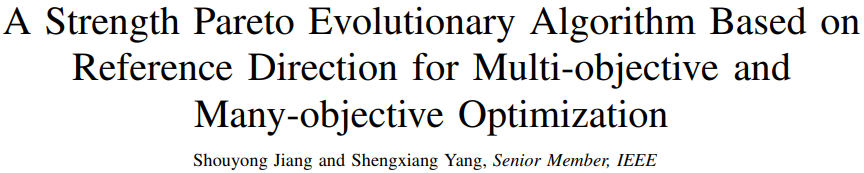
\includegraphics[scale=1]{artigo}
\end{center}

\section{Introdução}

\vspace{6mm}

\begin{itemize}
  \item Definições: Seja $M=$ o número de objetivos
  \item MOP = Multiobjective Optimization Problem --- $M \le 3$
  \item MaOP = Many-objective Optimization Problem --- $M \ge 4$
  \item Objetivo: Solucionar problemas anteriores, que surgem a partir de $4$ objetivos
  \item MOEA = Multiobjective Evolutionary Algorithm --- O desempenho cai drasticamente com o número de objetivos
  \item Também diminui a proporção de soluções não dominadas --- Acima de $10$ objetivos, quase todas as soluções são não dominadas
  \item Proposta: SPEA/R = Strength Pareto evolutionary algorithm (SPEA) based on reference direction
  \item Temos como um de nossos objetivos --- Melhorar a uniformidade das soluções
  \item Vamos utilizar --- um estimador de densidade, um novo esquema de atribuição de aptidão e uma nova estratégia de seleção ambiental
  \item Seja POS = Pareto-optimal set
  \item POF = Pareto-optimal front
  \item Vamos comparar com algoritmos pré-existentes --- $2$ de MOPs e $5$ de MaOPs
  \item Algoritmo $1$ --- HypE --- Emprega a métrica de hipervolume como um indicador na seleção ambiental; usa Simulação de Monte Carlo para aproximar o hipervolume exato;
  \item Algoritmo $2$ --- MOEA/D --- Visto em aula (decompõe um problema de otimização multiobjetivo em $N$ subproblemas de otimização escalar)
  \item Algoritmo $3$ --- NSGA-II --- Visto em aula (Algoritmo Genético de Classificação Não Dominado)
  \item Algoritmo $4$ --- PICEA-g --- Algoritmo coevolutivo baseado em preferências (PICEA), que co-evolui uma família de preferências do tomador de decisão junto com uma população de soluções candidatas, para otimização de muitos objetivos
  \item No PICEA-g as preferências ganham mais aptidão se esta for satisfeita por menos soluções, e as soluções ganham aptidão atendendo ao maior número de preferências possível
  \item Algoritmo $5$ --- SPEA2 --- Visto em sala
  \item A maioria dos MOEAs existentes adota uma estratégia de seleção de convergência em primeiro lugar e diversidade em segundo
  \item Vamos fazer o contrário --- Diversidade em primeiro lugar e convergência em segundo
\end{itemize}

\newpage

$\,$

\vspace{60mm}

\begin{itemize}
  \item O SPEA/R herda a vantagem da atribuição de aptidão do SPEA2 na quantificação da diversidade e na convergência das soluções em uma forma compacta
  \item Vamos substituir o estimador de densidade mais demorado por uma estimativa baseada em direção de referência
  \item Nossa atribuição de aptidão levará em consideração tanto convergência local quanto global
  \item O desempenho foi validado --- Foram feitos testes com problemas adequados
  \item Como o artigo é extenso, pretendo testar os algoritmos e fazer umas poucas comparações
  \item Até agora, fiz $1$ teste com $20$ pontos, mas ainda estou sem saber como interpretar
\end{itemize}

\newpage
\section{Algoritmo SPEA/R Proposto}

\vspace{6mm}

\begin{center}
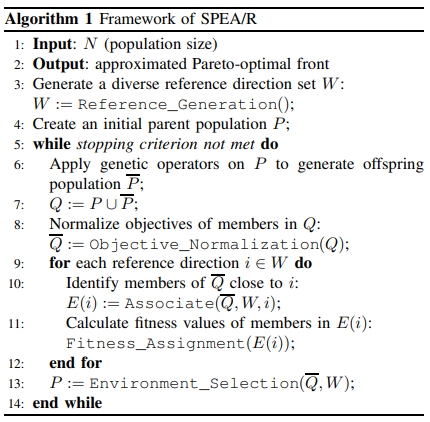
\includegraphics[scale=1]{alg1}
\end{center}

\begin{enumerate}[label=(\arabic*), itemsep=0mm]
  \item Gerar população inicial
  \item Construção de um conjunto predefinido de direções de referência
  \item Particionar o espaço de objetivos em várias sub-regiões independentes, para busca em direção a toda a POF com uma boa garantia de diversidade populacional no espaço de objetivos
  \item Para cada ciclo geracional, aplicar o operador genético para reproduzir uma população descendente (linha 6)
\end{enumerate}

\begin{center}
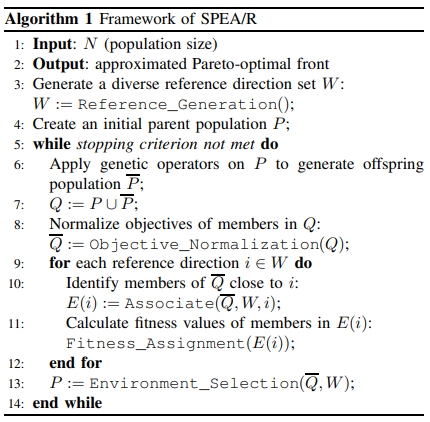
\includegraphics[scale=1]{alg1}
\end{center}

\begin{enumerate}[label=(\arabic*), itemsep=0mm]
  \setcounter{enumi}{4}
  \item União das populações ascendentes e descendentes, fusão das duas populações (linha 7)
  \item Normalização dos objetivos, para tornar o SPEA/R capaz de lidar com problemas com objetivos em escalas diferentes (linha 8)
  \item Cada membro da população combinada está associado a uma direção de referência (ou uma sub-região, linha 10)
  \item Dessa forma, os membros da população combinada são distribuídos em diferentes sub-regiões
\end{enumerate}

\begin{center}
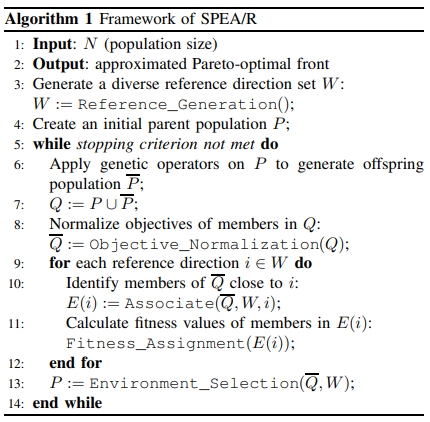
\includegraphics[scale=1]{alg1}
\end{center}

\begin{enumerate}[label=(\arabic*), itemsep=0mm]
  \setcounter{enumi}{8}
  \item Uma nova técnica de atribuição de aptidão é aplicada em indivíduos que residem em cada sub-região (linha 11)
  \item Uma estratégia de seleção de diversidade primeiro, convergência segundo, é adotada para construir uma nova população de pais para a próxima geração (linha 13)
\end{enumerate}

\newpage
\section{Geração do Conjunto de Direções de Referência}
\singlespacing

\vspace{6mm}

\begin{center}
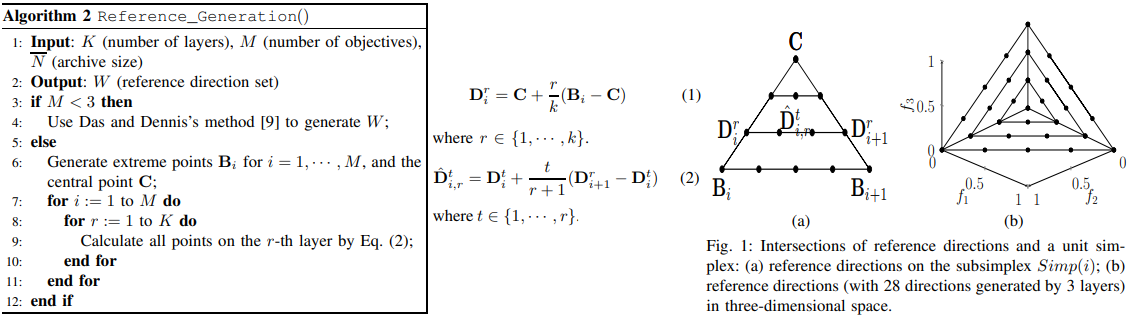
\includegraphics[scale=1.2]{alg2}
\end{center}

\begin{enumerate}[label=(\arabic*), itemsep=0mm]
  \item Seja: População ascendente = Arquivo
  \item Das and Dennis $=(\beta, 1 - \beta)$ --- Dividem $[0,1]^2$ em $p^2$ partes iguais
  \item Para problemas de alta dimensão, gera uma grande quantidade de direções de referência $= \begin{pmatrix} p + M - 1 \\ M - 1 \end{pmatrix}$, em que $p=$ o número de divisões em cada coordenada
  \item Construa o simplex ou tetraedro $i,j,k,\left(\cfrac{1}{3},\cfrac{1}{3},\cfrac{1}{3}\right)$; divida as arestas em $k$ partes; trace paralelas às arestas; divida cada paralela em $r + 1$ partes ; cada uma com $r$ pontos
\end{enumerate}

\doublespacing
\newpage
\section{Reprodução Descendente}

\vspace{6mm}

\begin{center}
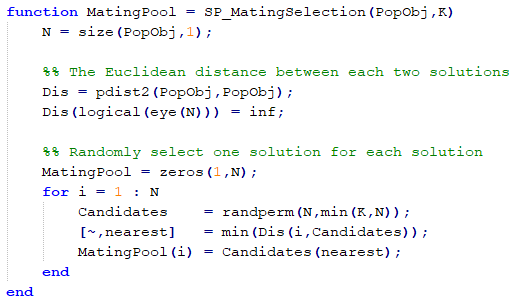
\includegraphics[scale=1.2]{MatingSelection}
\end{center}

\begin{enumerate}[label=(\arabic*), itemsep=0mm]
  \item ``Seleção de Acasalamento'' --- Cada indivíduo dos ascendentes $P_1$ precisa de um parceiro $P_2$ para fazer reprodução
  \item $K$ candidatos diferentes de $P_1$ são escolhidos aleatoriamente da população ascendente
  \item O candidato que minimiza a distância euclideana (no espaço de objetivos) até $P_1$ é incluído em $P_2$
  \item $K = 20$ é recomendado --- Veremos experimentalmente por quê
  \item Como aprimoramento, após a execução deste algoritmo, podemos utilizar cruzamento binário simulado (SBX) e mutação polinomial, como um dos possíveis ``operadores genéticos para gerar população descendente''
\end{enumerate}

\newpage
\section{Normalização dos Objetivos}

\vspace{6mm}

\begin{center}
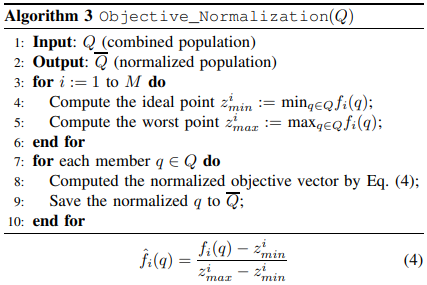
\includegraphics[scale=1.4]{alg3}
\end{center}

\begin{itemize}
  \item Visto em aula
\end{itemize}

\newpage
\section{Associação de Membros}

\vspace{6mm}

\begin{center}
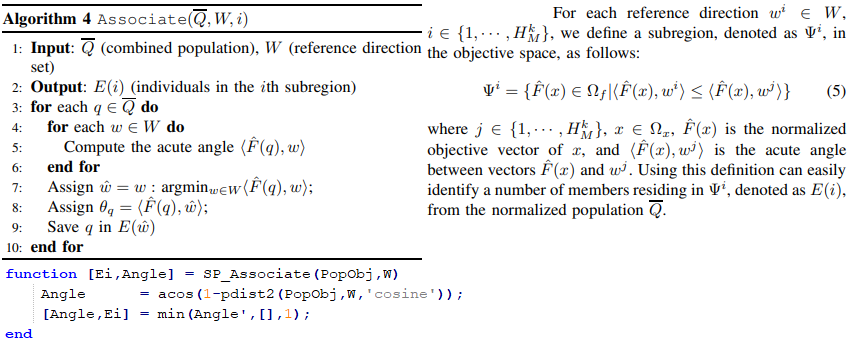
\includegraphics[scale=1.35]{alg4}
\end{center}

\begin{itemize}
  \item Seja $H^k_M=$ cardinalidade de direções de referência, $k=$ número de camadas do simplex ou tetraedro
\end{itemize}

\newpage
\section{Atribuição de Aptidão}

\vspace{6mm}

\begin{center}
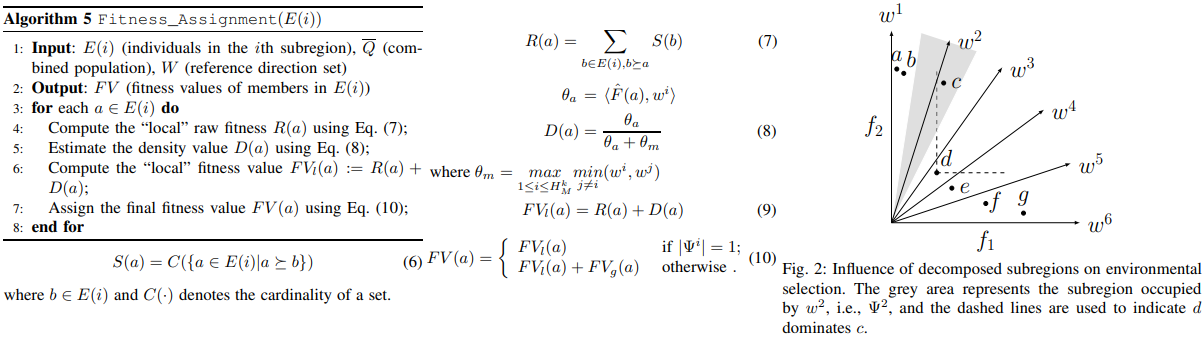
\includegraphics[scale=1.125]{alg5}
\end{center}

\begin{itemize}
  \item $FV_g(a)$ é igual à aptidão bruta do SPEA2
  \item O objetivo é dar uma chance às regiões que têm um único ponto --- As quais outros algoritmos descartam
\end{itemize}

\newpage
\section{Seleção Ambiental}

\vspace{6mm}

\begin{center}
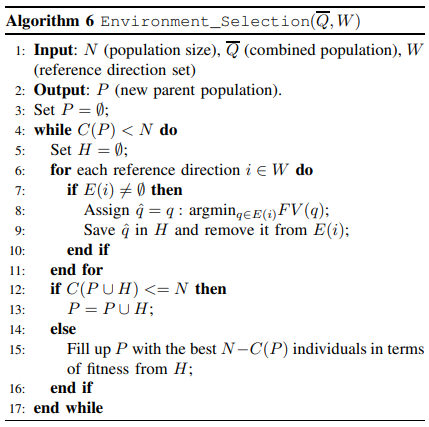
\includegraphics[scale=1]{alg6}
\end{center}

\begin{enumerate}[label=(\arabic*), itemsep=0mm]
  \item Os melhores $N$ indivíduos que podem equilibrar diversidade e convergência devem ser preservados
  \item Selecionar repetidamente uma matriz $H$ de indivíduos vindos de cada sub-região
  \item Copiar os indivíduos selecionados para a nova população $P$ se o tamanho da população $C(P)$ não for maior do que $N$ (linha 13)
  \item Caso contrário, $H$ é classificado de acordo com a aptidão dos indivíduos (linhas 8-9), e, em seguida, os melhores $N - C(P)$ indivíduos são copiados para $P$ (linha 15)
\end{enumerate}

\begin{center}
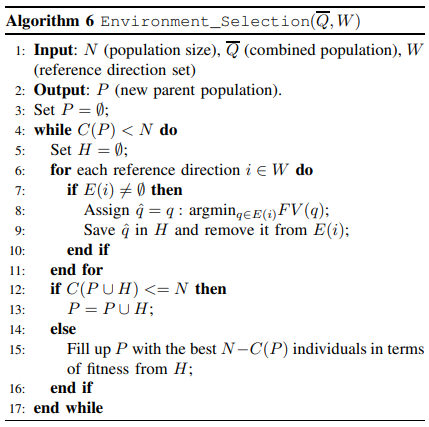
\includegraphics[scale=1]{alg6}
\end{center}

\begin{enumerate}[label=(\arabic*), itemsep=0mm]
  \setcounter{enumi}{4}
  \item Indivíduos na primeira execução do loop de seleção (linhas $6-11$) têm a maior diversidade
  \item E aqueles no segundo loop têm a segunda maior diversidade, e assim por diante. Dessa forma, a diversidade da população pode ser bem mantida
  \item A estratégia de seleção pode ser aprimorada pela elaboração da contagem de nicho de cada sub-região ao realizar a seleção de convergência (linha $15$) para preencher $P$
\end{enumerate}

%\newpage

%$\,$

%\vspace{60mm}

%\section{Complexidade Computacional do SPEA/R}

%\vspace{6mm}

%\begin{itemize}
%  \item A complexidade média de um ciclo geracional do SPEA/R é $O(MN^2)$
%  \item O pior caso é: todos os $2N$ indivíduos ficam presos em uma sub-região e as outras sub-regiões não contêm nenhum membro
%  \item Nesse caso, a complexidade computacional chega a $O(MN^2)$, que é igual à complexidade média
%\end{itemize}

\newpage
\section{Experimentos --- Otimização Multiobjetivo}

\vspace{6mm}

\begin{itemize}
  \item $M \le 3$
  \item Compara o SPEA/R com os dois algoritmos abaixo:
  \item Algoritmo $6$ --- MOEA/D-M2M --- Otimização evolutiva multiobjetivo baseada em decomposição. Este algoritmo resolve subproblemas de forma colaborativa. Cada subproblema tem sua própria população e recebe esforço computacional a cada geração. Dessa forma, a diversidade da população pode ser mantida.
  \item Algoritmo $7$ --- MOEA/D-ACD --- Impõe restrições aos subproblemas. Ajusta de forma adaptativa as restrições usando informações coletadas na pesquisa.
  \item A comparação utiliza Métricas de Desempenho
  \item IGD = Distância Geracional Invertida --- Calcule a distância de cada ponto $p$ da POF Aproximada até a POF Verdadeira inteira (mínimo sobre $V$); Divida pela cardinalidade de $V$ ; Compare o IGD dos algoritmos
  \item HV = Hipervolume abaixo do referencial = $(2, 2, ..., 2)$ ; Compare o HV dos algoritmos
  \item Nestes experimentos, é utilizado o conjunto de testes MOP --- $7$ fronteiras dos autores H-L Liu, F. Gu, Q. Zhang
  \item Uma vez que é necessário gerar uma POF Verdadeira, com pontos uniformemente distribuídos
  \item Cada algoritmo para após $300, 600, 1000, 1500$, e $2000$ gerações para os casos de $2, 3, 5, 8, 12$ objetivos
  \item Foram feitas $30$ execuções independentes em cada instância de teste
\end{itemize}

\newpage

$\,$

\vspace{60mm}

\begin{itemize}
  \item Resultados --- Tabela de Desempenho --- SPEA/R ganha de MOEA/D-M2M e MOEA/D-ACD --- IGD e HV --- MOP1 a MOP7
\end{itemize}

\begin{center}
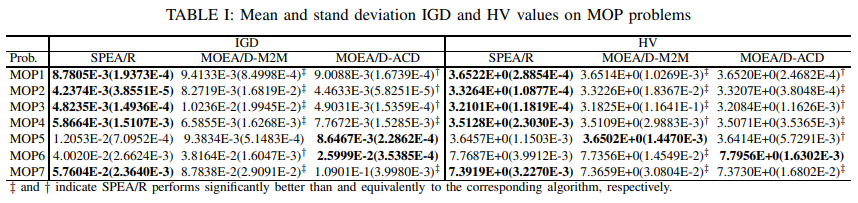
\includegraphics[scale=1.2]{table1}
\end{center}

\newpage

\begin{itemize}
  \item Gráficos das Fronteiras $f_1$, $f_2$, $f_3$, MOP4 a MOP7 --- SPEA/R uniforme, MOEA/D-M2M intermediário, MOEA-D/ACD pouco uniforme
\end{itemize}

\begin{center}
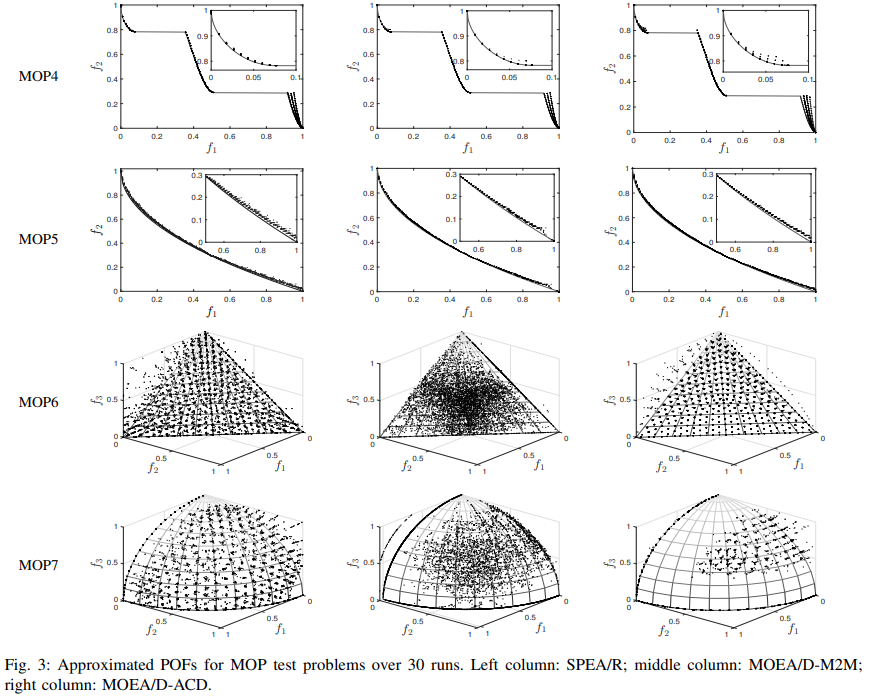
\includegraphics[scale=0.9]{fig3}
\end{center}

\newpage
\section{Experimentos --- Otimização de Muitos Objetivos}

\vspace{6mm}

\begin{itemize}
  \item $M \ge 4$
  \item Nestes experimentos, é utilizado o conjunto de ferramentas WFG = Walking Fish Group --- Dos autores S. Huband, P. Hingston, L. Barone, L. While
  \item Compara o SPEA/R com os cinco algoritmos abaixo:
  \item MOEA/D de novo
  \item HypE de novo
  \item Algoritmo $8$ --- SPEA2+SDE --- Introduz um estimador de densidade que considera a distribuição e a convergência de informações dos indivíduos para aumentar a pressão de seleção na otimização de muitos objetivos
  \item PICEA-g de novo
  \item Algoritmo $9$ --- NSGAIII --- Versão atualizada do NSGA-II baseada em dominância, em que uma série de pontos de referência fornecidos são usados como uma diretriz para lidar com MaOPs; Mantém a diversidade da população por meio da preservação de nicho
\end{itemize}

\newpage

\begin{itemize}
  \item Resultado de Desempenho --- SPEA/R ganha em IGD --- WFG1 a WFG9 --- $M = 2,3,5,8,12$
\end{itemize}

\begin{center}
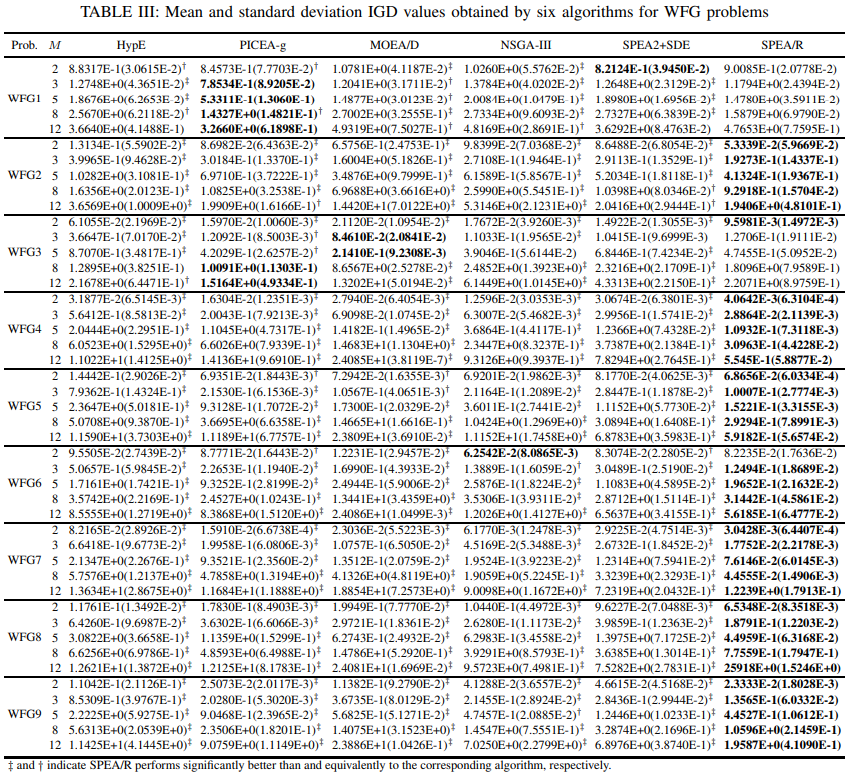
\includegraphics[scale=0.85]{table3}
\end{center}

\newpage

\begin{itemize}
  \item Resultado de Desempenho --- SPEA/R ganha em HV --- WFG1 a WFG9 --- $M = 2,3,5,8,12$
\end{itemize}

\begin{center}
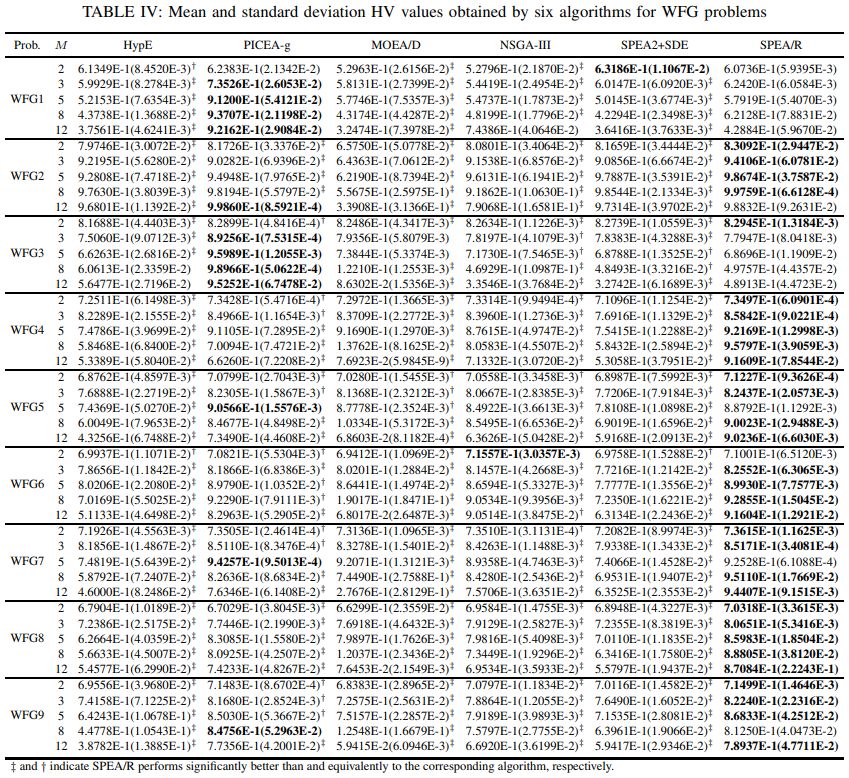
\includegraphics[scale=0.85]{table4}
\end{center}

\newpage

$\,$

\vspace{20mm}

\begin{itemize}
  \item Plotar graficamente as coordenadas paralelas (normalizadas) das soluções finais obtidas por cada algoritmo
  \item SPEA/R ganha em uniformidade
\end{itemize}

\begin{center}
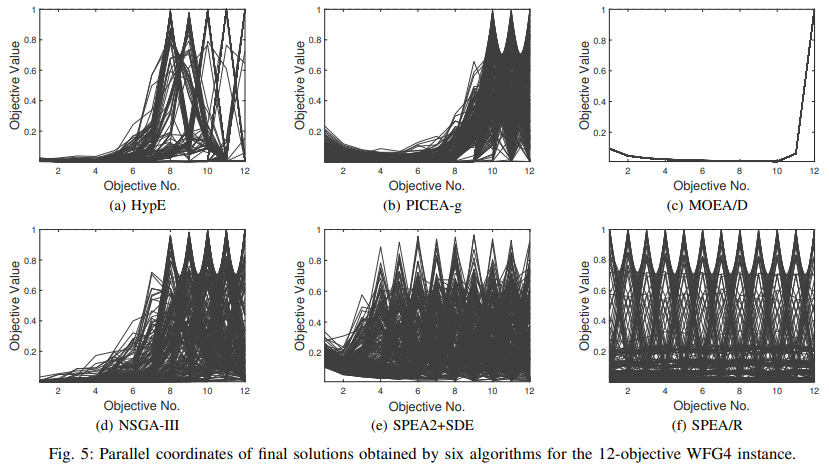
\includegraphics[scale=1]{fig5}
\end{center}

\newpage

\begin{itemize}
  \item SPEA/R ganha em Tamanho da População
  \item Comparação de diferentes abordagens de geração de direção de referência
  \item Gráfico do Tamanho da amostra $\times$ Tamanho da população, $M = 3, 5, 7, 8, 15, 30$ --- Comparação com NSGAIII
  \item No eixo $x$, temos $n \cdot H^k_M=$ quantas vezes o número de direções de referência
  \item No último caso, a comparação é entre $10^3$ com $10^5$ de população
\end{itemize}

\begin{center}
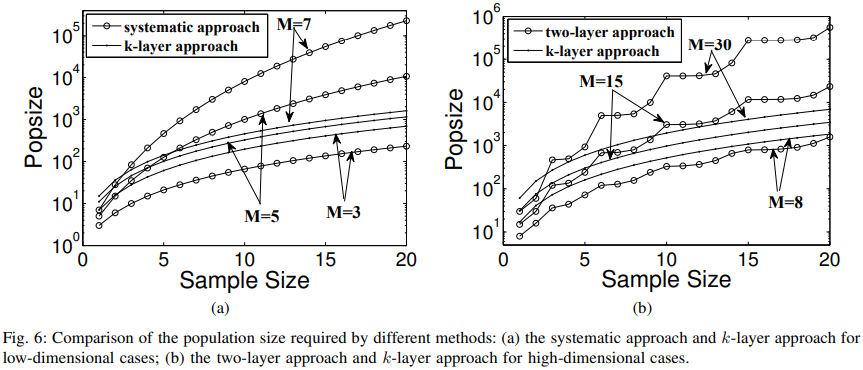
\includegraphics[scale=1]{fig6}
\end{center}

\newpage

\begin{itemize}
  \item Gráfico das Fronteiras em Escala $f_1$, $f_2$, $f_3$, WFG5 --- Comparação com NSGAIII
  \item Os objetivos $f_1$, $f_2$, $f_3$ estão multiplicados por $5, 5^2, 5^3$, respectivamente
  \item SPEA/R ganha em uniformidade
\end{itemize}

\begin{center}
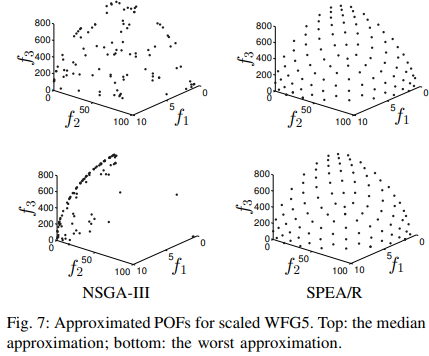
\includegraphics[scale=1.2]{fig7}
\end{center}

\newpage

\begin{itemize}
  \item Influência do acasalamento restrito --- Desempenho --- $K = 20$ minimiza o HV, WFG5 a WFG8, $M = 2,3,5,8,12$
\end{itemize}

\begin{center}
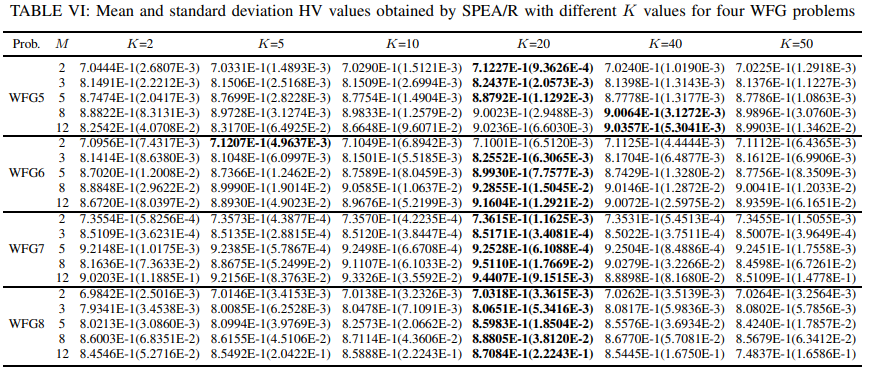
\includegraphics[scale=1]{table6}

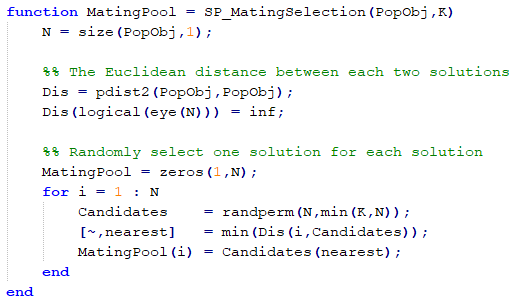
\includegraphics[scale=1]{MatingSelection}
\end{center}

\newpage

$\,$

\vspace{30mm}

\begin{itemize}
  \item Influência do acasalamento restrito --- Plotar graficamente as coordenadas paralelas (normalizadas) das soluções finais --- WFG4, $M = 20, 40$
  \item Novamente a uniformidade da fronteira do SPEA/R
\end{itemize}

\begin{center}
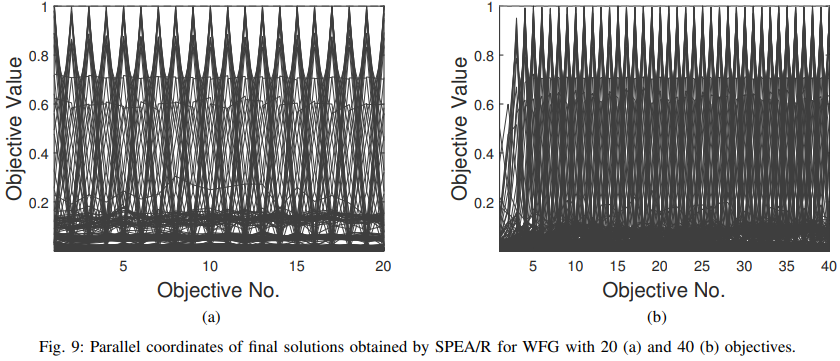
\includegraphics[scale=1]{fig9}
\end{center}

\newpage

$\,$

\vspace{30mm}

\begin{itemize}
  \item Gráfico Gerações $\times$ Percentual de soluções dominadas, WFG5
  \item O SPEA/R prioriza a geração de soluções não dominadas 
\end{itemize}

\begin{center}
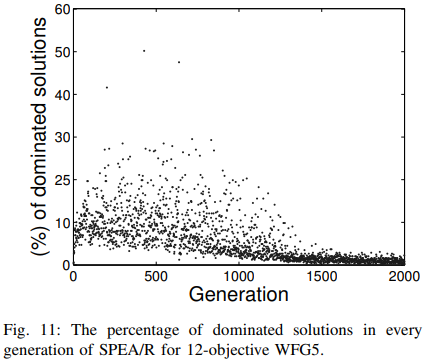
\includegraphics[scale=1]{fig11}
\end{center}

\newpage
\section{Conclusões}

\vspace{6mm}

\begin{itemize}
  %\item MOEAs convencionais baseados em dominância de Pareto podem ser inadequados para muitos objetivos de otimização
  %\item Apesar de que eles possam resolver com sucesso problemas de dois ou três objetivos
  \item O SPEA/R resolve tanto MOPs quanto MaOPs
  %\item O SPEA/R particiona o espaço objetivo em várias sub-regiões de interesse
  %\item E os indivíduos em cada sub-região são guiados para direções de pesquisa predefinidas
  %\item O SPEA/R adota uma estratégia de seleção de diversidade em primeiro lugar e convergência em segundo
  %\item O que pode aumentar a pressão de seleção para otimização de muitos objetivos, em que uma grande fração da população é não dominada
  %\item O SPEA/R também emprega um esquema de acasalamento restrito para melhorar a eficiência da reprodução
  \item A estrutura proposta reduziu significativamente o esforço computacional de métodos baseados em SPEA, com complexidade computacional limitada por $O(MN^2)$
  %\item O estudo experimental demonstrou a eficácia do SPEA/R em uma série de problemas de teste MOP e WFG com $2$ a $40$ objetivos e várias dificuldades de otimização
  \item Uma comparação justa com vários MOEAs de última geração sugere que o SPEA/R é muito superior para otimização multiobjetivo e de muitos objetivos
  \item Mas não a maior qualidade possível 
  \item Dar alta prioridade à diversidade em vez da convergência pode ser outra maneira eficaz de lidar com a otimização de muitos objetivos
  \item O SPEA/R precisa ser examinado em uma gama mais ampla de problemas (por exemplo, formas complicadas de POS e POF)
  \item Questões em aberto, como por exemplo o cálculo computacionalmente caro das métricas de desempenho
  \item E a visualização de fronteiras em dimensões mais elevadas
  \item Portanto, esses devem ser tópicos muito interessantes para trabalho futuro
\end{itemize}

\newpage
\section{Referências}

\vspace{6mm}

\begin{itemize}
  \item $[40]$ R. L. While, L. Bradstreet, and L. Barone, “A fast way of calculating exact \textbf{hypervolumes},” IEEE Trans. Evol. Comput., vol. 16, no. 1, pp. 86–95, 2012.
  \item \textbf{Sobre MOPs e MOEA/D-M2M:} $[34]$ H. Liu, F. Gu, and Q. Zhang, “Decomposition of a multiobjective optimization problem into a number of simple multiobjective subproblems,” IEEE Trans. Evol. Comput., vol. 18, no. 3, pp. 450–455, 2014.
  \item \textbf{Sobre WFG:} $[21]$ S. Huband, P. Hingston, L. Barone, and L. While, “A review of multiobjective test problems and a scalable test problem toolkit,” IEEE Trans. Evol. Comput., vol. 10, no. 2, pp. 477–506, 2006.
  \item \textbf{Sobre MOEA/D-ACD:} $[44]$ L. Wang, Q. Zhang, A. Zhou, M. Gong, and, L. Jiao, “Constrained subproblems in decomposition based multiobjective evolutionary algorithm,” IEEE Trans. Evol. Comput., vol. 20, no. 3, pp. 475–480, 2015.
  \item $[4]$ J. Bader and E. Zitzler, “\textbf{HypE:} An algorithm for fast hypervolume-based many-objective optimization,” Evol. Comput., vol. 19, no. 1, pp. 45–76, 2011.
  \item \textbf{Sobre SPEA2+SDE:} $[32]$ M. Li, S. Yang, X. Liu, “Shift-based density estimation for Pareto-based algorithms in many-objective optimization,” IEEE Trans. Evol. Comput., vol. 18, no. 3, pp. 348–365, Jun. 2014.
  \item \textbf{Sobre PICEA-g:} $[43]$ R. Wang, R. C. Purshouse, and P. J. Fleming, “Preference-inspired coevolutionary algorithms for many-objective optimization,” IEEE Trans. Evol. Comput., vol. 17, no. 4, pp. 474–494, Aug. 2013.
  \item \textbf{Sobre NSGA3:} $[13]$ K. Deb and H. Jain, “An evolutionary many-Objective optimization algorithm using reference-point based non-dominated sorting approach, Part I: Solving problems with box constraints,” IEEE Trans. Evol. Comput., vol. 18, no. 4, pp. 577–601, 2014.
\end{itemize}

\newpage

$\,$

\vspace{60mm}

\begin{itemize}
  \item \textbf{Sobre Reference Generation:} $[9]$ I. Das and J. Dennis, “Normal-boundary intersection: A new method for generating the Pareto surface in nonlinear multicriteria optimization problems,” SIAM J. Optimiz., vol. 8, no. 3, pp. 631–657, 1998.
  \item \textbf{Sobre cruzamento binário simulado (SBX) e mutação polinomial:} $[55]$ Yuan J, Liu HL, Gu F (2018) A cost value based evolutionary manyobjective optimization algorithm with neighbor selection strategy. In: 2018 IEEE congress on evolutionary computation (CEC). IEEE, pp 1–8
\end{itemize}

\newpage

\Huge

\onehalfspacing

$\,$

\vspace{70mm}

\begin{center}
\textbf{OBRIGADO.}
\end{center}

\vspace{70mm}

\normalsize

Fora da caridade, não há salvação. Com caridade, há evolução.

Vinicius Claudino Ferraz, versão de 07/janeiro/2022.

\end{document}
